\section{Results}

\subsection{Criterion conflict is unavoidable in every domain}

\begin{table}[t]
\centering
\caption{Conflict bound $B$ and the exact scalar minimum $B_{\mathrm{exact}}$
(all 720 orderings per image) on the eight panels.}
\label{tab:conflict}
\scriptsize
\setlength{\tabcolsep}{1.7pt}
\begin{tabular}{lcccccccc}
\toprule
 & COCO & VOC & ADE-S & ADE-X & ADE-M & City & KITTI & CT \\
\midrule
$B$ & \NBCoco & \NBVoc & \NBAdeS & \NBAdeX & \NBAdeM & \NBCity & \NBKitti & \NBAmos \\
$B_{\mathrm{exact}}$ & \NBExactCoco & \NBExactVoc & \NBExactAdeS & \NBExactAdeX & \NBExactAdeM & \NBExactCity & \NBExactKitti & \NBExactAmos \\
\bottomrule
\end{tabular}
\end{table}

\begin{figure*}[t]
  \centering
  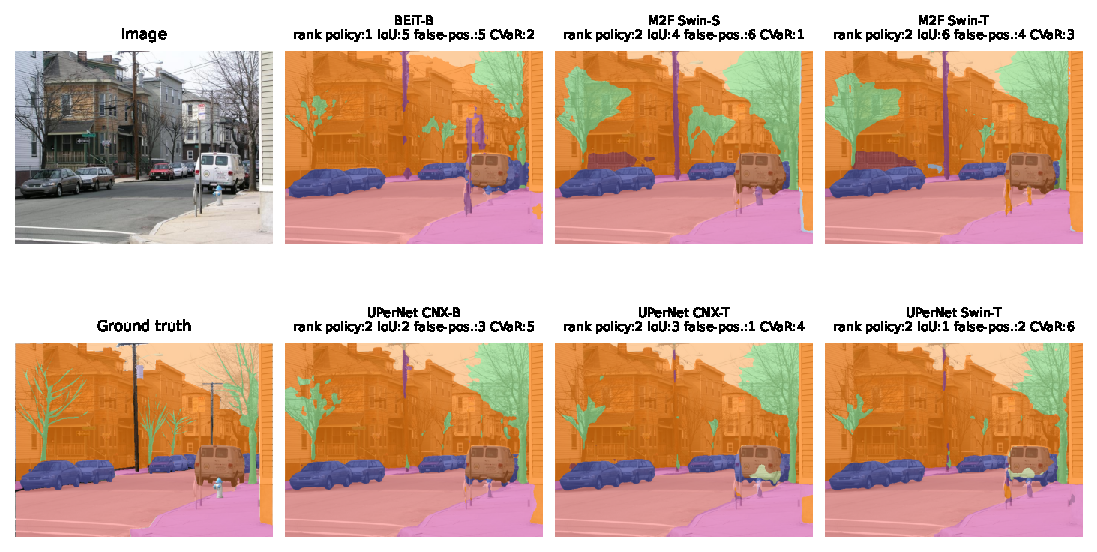
\includegraphics[width=0.92\textwidth]{qualitative.pdf}
  \caption{Real predictions of the six ADE-X models on one validation image,
  with each model's rank (1 = best; ties share a rank) under four of the seven
  criteria. The image was chosen by a fixed rule: among ADE-X images containing
  a critical component, with non-constant policy utility across models and at
  least 60 non-tied criterion votes, the one with the largest per-image exact
  conflict. No ordering of these six models agrees with all criteria.}
  \label{fig:qualitative}
\end{figure*}

The bound is positive on all eight panels (Table~\ref{tab:conflict},
Fig.~\ref{fig:qualitative}), from
\NBAllMin{} on Cityscapes to \NBAllMax{} on KITTI, and the exact minimum exceeds
it by at most \NBGapAllMax{}. Intransitive preference cycles therefore add
almost nothing: the conflict is pairwise and no scalar can remove it. On the
general-scene panels, leave-one-criterion-out lower confidence limits are at
least \NOneLooMinLow{}, counting ties as agreement lowers the bound to at least
\NOneTieAgreeMin{}, splitting ties raises it to at most \NOneTieSplitMax{}, and
across all three-model subsets of ADE-M the bound ranges from
\NOneSubsetMinAdeM{} to \NOneSubsetMaxAdeM. Its size depends on which criteria
are declared: deployment-only criteria give \NOneBDeployAdeS{}--\NOneBDeployAdeX{}
on ADE20K, versus \NOneBConvAdeS{}--\NOneBConvAdeX{} after adding the overlap
criteria.

\subsection{Endpoint-specific scoring transfers across domains}

\begin{figure*}[t]
  \centering
  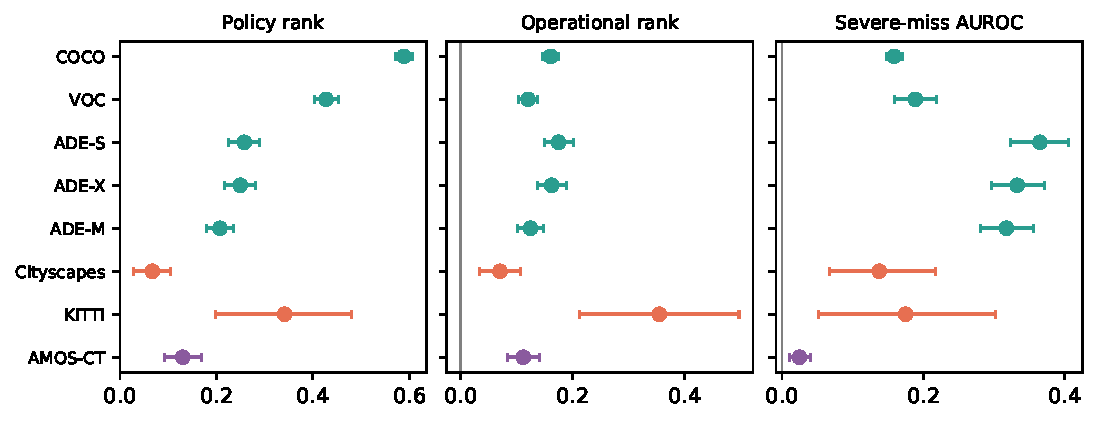
\includegraphics[width=0.94\textwidth]{gains_forest.pdf}
  \caption{Endpoint-specific score minus reuse of the mixed score on all eight
  panels (95\% paired image-cluster bootstrap intervals). Teal: general scenes;
  orange: street scenes; purple: abdominal CT. All contrasts remain significant
  after Holm correction over \NFamilyN{} tests.}
  \label{fig:gains}
\end{figure*}

Scoring each endpoint with its own frozen formula improves policy-rank
agreement, operational-rank agreement, and severe-miss AUROC on every panel
(Fig.~\ref{fig:gains}). All \NNontrivialSig{} of \NNontrivialN{} contrasts are
significant after Holm correction over all \NFamilyN{} panel-by-endpoint tests
(largest adjusted $p=\NNontrivialMaxHolm$), and the smallest lower confidence
limit is \NMinGainLow. The gains hold on panels never used for selection: recent
ADE20K architectures (\NGPolAdeM{} in policy rank, \NGSevAdeM{} in severe-miss
AUROC), street scenes (\NGPolKitti{} and \NGSevKitti{} on KITTI), and CT
(\NGPolAmos{} and \NGSevAmos).

\paragraph{Robustness.} On the four original general-scene panels, re-running
the full 260-formula selection on resampled COCO and VOC images in each of
1,000 bootstrap draws leaves \NOneNestedAllPos{} of \NOneNestedAllN{} contrasts
with intervals above zero, so the advantage does not depend on the particular
formulas chosen. With the formulas frozen, the contrasts stay positive with
intervals excluding zero under uniform priorities, all \NOnePrioSingleN{}
single-class priority changes, and \NOnePrioPermN{} random permutations of
priority values. Recomputing AUROC exactly in each draw changes interval limits
by at most \NOneExactLinMaxDiff{} relative to an influence-function
approximation, and under a paired-exchange null the test rejects at
\NOneNullRateMin{}--\NOneNullRateMax{} at nominal level 0.05.

\paragraph{Human judgments.}\label{sec:human} To obtain an endpoint not built
from the scores' own components, \NHumAnnotators{} reviewers, blind to models and
scores, compared 100 pairs of real ADE-X predictions on which the
endpoint-specific policy score and the mixed score disagree, answering one fixed
question: which segmentation covers people and vehicles better. Protocol and
analysis were pre-registered. On the \NHumPairs{} pairs with a clear majority,
the majority sided with the endpoint-specific score on \NHumAgree\% (95\%
image-cluster bootstrap CI [\NHumLo, \NHumHi]\%; one-sided $p=\NHumP$) and with
the mixed score on \NHumAgreeMixed\%; inter-rater agreement was moderate
(Fleiss' $\kappa=\NHumKappa$). Among single criteria, policy utility matched the
majority most often (\NHumPolicy\%) and false-positive quality least
(\NHumFp\%). The effect is moderate, and on control pairs where both scores
agree the majority matched them only \NHumControl\% of the time, so the study
supports the comparison between the two scores rather than close agreement of
either with human judgment.

\subsection{A single failure score depends on failure composition}

\begin{figure*}[t]
  \centering
  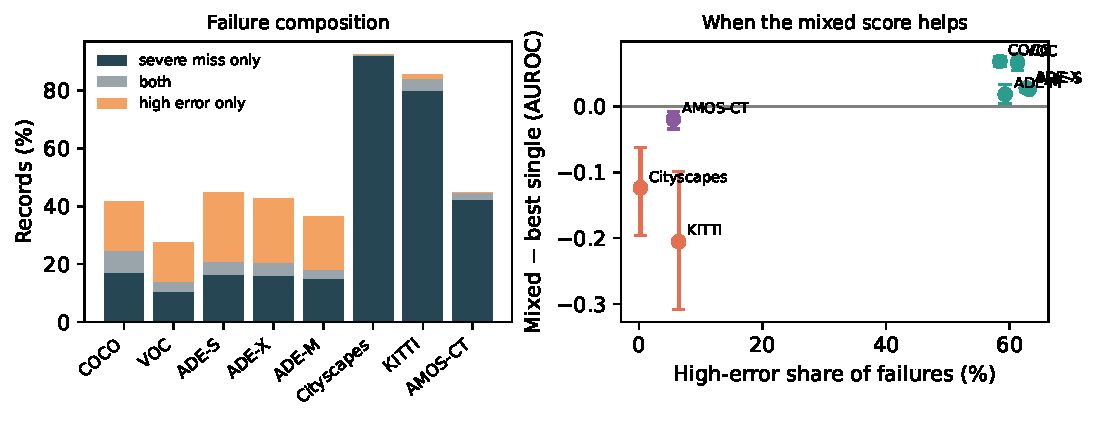
\includegraphics[width=0.96\textwidth]{composition_gap.pdf}
  \caption{Left: composition of failure records on each panel. Right: frozen
  mixed failure score minus the strongest single metric (mixed-failure AUROC,
  95\% CI) against the share of failures involving high error.}
  \label{fig:composition}
\end{figure*}

\begin{table*}[t]
\centering
\caption{Mixed-failure AUROC. High: high-error share of failures. Frozen:
general-scene mixed score minus the strongest single metric. Matched: score
re-selected on Cityscapes training data, minus the frozen mixed score and
minus the strongest single metric (95\% CI).}
\label{tab:composition}
\footnotesize
\setlength{\tabcolsep}{4pt}
\begin{tabular}{lcccc}
\toprule
Panel & High (\%) & Frozen $-$ best & Matched $-$ frozen & Matched $-$ best \\
\midrule
COCO & \NHighShareCoco & \NMvbCoco{} [\NMvbLoCoco, \NMvbHiCoco] & -- & -- \\
VOC & \NHighShareVoc & \NMvbVoc{} [\NMvbLoVoc, \NMvbHiVoc] & -- & -- \\
ADE-S & \NHighShareAdeS & \NMvbAdeS{} [\NMvbLoAdeS, \NMvbHiAdeS] & -- & -- \\
ADE-X & \NHighShareAdeX & \NMvbAdeX{} [\NMvbLoAdeX, \NMvbHiAdeX] & -- & -- \\
ADE-M & \NHighShareAdeM & \NMvbAdeM{} [\NMvbLoAdeM, \NMvbHiAdeM] & -- & -- \\
\midrule
City & \NHighShareCity & \NMvbCity{} [\NMvbLoCity, \NMvbHiCity] & \NSelGainCity{} [\NSelGainLoCity, \NSelGainHiCity] & \NSelBestCity{} [\NSelBestLoCity, \NSelBestHiCity] \\
KITTI & \NHighShareKitti & \NMvbKitti{} [\NMvbLoKitti, \NMvbHiKitti] & \NSelGainKitti{} [\NSelGainLoKitti, \NSelGainHiKitti] & \NSelBestKitti{} [\NSelBestLoKitti, \NSelBestHiKitti] \\
CT & \NHighShareAmos & \NMvbAmos{} [\NMvbLoAmos, \NMvbHiAmos] & \NSelGainAmos{} [\NSelGainLoAmos, \NSelGainHiAmos] & \NSelBestAmos{} [\NSelBestLoAmos, \NSelBestHiAmos] \\
\bottomrule
\end{tabular}
\end{table*}

The general-scene mixed score, $h_{\mathrm{mixed}}=0.2\,q_{\mathrm{comp}}+0.8\,q_{\mathrm{fp}}$,
is the best failure detector on all five general-scene panels, with every
interval above zero, and trails the strongest single metric on all three
street-scene and CT panels, with every interval below zero
(Table~\ref{tab:composition}). The strongest single metric there is a coverage
or tail score: \NMvbNameCity{} on Cityscapes and KITTI and \NMvbNameAmos{} on CT.
The two groups differ in failure composition (Fig.~\ref{fig:composition}): on
general scenes high-error failures make up \NMinShareWin{}--\NMaxShareWin\% of
failures, on street scenes and CT at most \NMaxShareLose\%. The advantage of the
mixed score also varies with the high-error threshold on general scenes,
positive in \NOneThrPosVoc{}/7 VOC cells, \NOneThrPosCoco{}/7 COCO cells, and
\NOneThrPosAdeS{}/7 cells on each of ADE-S and ADE-X.

In street scenes the residual failures are concentrated in small, distant
objects. On Cityscapes \NCitySevere\% of model--image records contain a severe
miss; in \NCityPersonShare\% of them the worst-covered critical component is a
person, with median size \NCityCulpritMedian{} pixels in a
\NCityImagePixels-pixel image, and \NCityCulpritBelowK\% of these components
cover fewer than 1,024 pixels. A 16-pixel eligibility rule set for
lower-resolution images admits these objects; as a sensitivity check only,
ignoring critical components below 4,096 pixels lowers the severe-miss rate to
\NCitySevereIgnoreFourK\%.

\paragraph{Domain-matched selection.} Re-selecting the failure score on
Cityscapes training records, in which severe misses vastly outnumber high-error
failures, yields $\NSelFirstWeight\,q_{\mathrm{arith}}+\NSelSecondWeight\,q_{\mathrm{fp}}$,
where $q_{\mathrm{arith}}$ is severity-weighted arithmetic coverage. On the three
held-out panels it beats the general-scene mixed score by \NSelGainCity{}
(Cityscapes validation), \NSelGainKitti{} (KITTI), and \NSelGainAmos{} (CT), all
significant after Holm correction (largest adjusted $p=\NSelMaxHolm$), and its
gap to the strongest single metric is no longer distinguishable from zero
(Table~\ref{tab:composition}). Matching the selection data to the failure
composition of the target domain thus restores the failure score, including on
CT, a domain absent from its selection data.
